\documentclass[12pt,oneside,letterpaper]{article}

\usepackage{graphicx}
\usepackage[font=small,labelfont=bf]{caption}
\pagestyle{headings}
\oddsidemargin 0.25in \textwidth     6.25in \topmargin     0.4in
\textheight    8.5in

\begin{document}


\title{\bfseries Data Classifier: \\
Software Architecture\\
Version 1.0}

\author {
\large{Team Mark}\\
\emph{Computer Science Department}\\
\emph{California Polytechnic State University}\\
\emph{San Luis Obispo, CA USA}\\
}

\date{November 7, 2018}
\maketitle \thispagestyle{empty}

\pagebreak
\tableofcontents

\addcontentsline{toc}{section}{Revision History}

\addcontentsline{toc}{section}{Credits}

\section*{Credits}
\begin{tabular}{|l|l|p{2.5in}|l|}
\hline
\textbf{Name}&\textbf{Date}&\textbf{Role}&\textbf{Version}\\
\hline
Matt Yamolich &November 7, 2018&Contributing Member&1.0\\
\hline
Spencer Schurk&November 7, 2018&Lead Author of Introduction&1.0\\
\hline
Sally Jones&October 10, 2009&Lead Author of Business Requirements&1.0\\
\hline
&&&\\
\hline
&&&\\
\hline
\end{tabular}

\section*{Revision History}
\begin{tabular}{|l|l|p{2.5in}|l|}
\hline
\textbf{Name}&\textbf{Date}&\textbf{Reason for Changes}&\textbf{Version}\\
\hline
Spencer Schurk&November 7, 2018&Completed Introduction&1.0\\
\hline
&&&\\
\hline
&&&\\
\hline
&&&\\
\hline
\end{tabular}

\newpage

\section{Introduction}

The purpose of this document is to describe the architecture of our Data Classifier. This document will be used as a reference when development begins. This document may change over time as we learn more about specific technologies being used for this project. For more information regarding this project, please see the Vision and Scope document, as well as the SRS document.

\section{Problem Description}
[Tell the audience what problem is being solved, or requirements are being met, by this design.  Include requirements or constraints that drive the direction of the design.

Any quality attribute requirements or constraints should also be explained in this section.]



\section{Solution}
This project is meant as an interface between a database and the data being inputted to it by the user. The main goal of this project is to provide analytics for the user in order to better identify what type of data is being inputted. With this project, the user will be able to tell the categories of data being inputted, and how they potentially relate to each other. The classifier will allow the user to modify these relations and to interact with a visual model based on these interactions. As defined by the customer, the user will interact with a web based GUI, most likely based on React. This GUI will interface with the Python backend, which is another design restraint, and utilize Scikit, a python library, as our chosen machine classifier. This classifier will act as the main interface/buffer between the user and actually logging the data to the database. 

\subsection{Overview}
[This section should be a summary of the solution in a few paragraphs, preferably less than a page.]

\subsection{Components}
[This section should list and briefly describe the components of the design.  The word ``components'' can refer to deployable units or to areas of the design, as appropriate. This section should start with the deployment diagram.]

\subsection{Design}
[This is where the meat of the design lives.  For each component, there should be a subsection describing the design of that component in as much detail as you want to provide in a high-level design.  There should also be a subsection that describes how the components work together. This section should include class, sequence, and collaboration diagrams as appropriate.]

\subsubsection{Classification Structure}
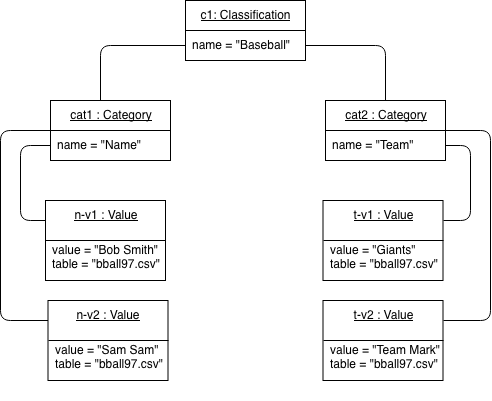
\includegraphics[scale = 0.9]{spencer_object.png}
\begingroup
\captionof{figure}{Data Classification Object Diagram - Spencer Schurk}
\endgroup

\paragraph{} Figure 1 depicts the architecture of our Classification object. Once data classification has completed on the provided files, the finalized result will be structured like this. A classification consists of one Classification object, which contains a String called name, and one to many Categories. 
\paragraph{} Categories are what the classified data is sorted into by the machine learning algorithms. A category consists of a String called name, and one to many values.
\paragraph{} Values are the object representation of one value in a data set. The Value object contains the value, and a reference to the table in which it came from. More attributes may be stored in the Value object as necessary.
\section{Test}
[This section should describe how the solution will be tested, especially if the test scenario or test infrastructure are complex.]

\section{Issues}
[Any issues or open questions should be described here.]

\appendix
\section{Glossary}
Define all the terms necessary to properly interpret the software architecture, including acronyms and abbreviations. You may wish to build a separate glossary that spans multiple projects or the entire organization, and just include terms specific to a single project in each software architecture.

\section{Issues List}
This is a dynamic list of the open architecture issues that remain to be resolved, including TBDs, pending decisions, information that is needed, conflicts awaiting resolution, and the like.
\end{document}
